\section{Design and Implementation\label{design}}

\begin{figure}
\center
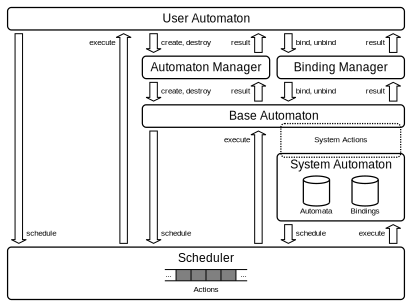
\includegraphics[width=\textwidth]{architecture}
\caption{Framework architecture.}
\label{framework_architecture}
\end{figure}

An implementation of the model described in section~\ref{component_model} must provide a service for executing local actions and facilities for manipulating the set of automata and bindings.
The architecture of our framework is depicted in Figure~\ref{framework_architecture}.
The Scheduler has the resposibility of selecting and executing local actions subject to the I/O automata model and concurrency constraints of~\ref{component_model}.
All user automata inherit from a common base class that provides facilities for asynchronously creating and destroying child automata and bindings.
The services provided by the base class are indicated by the Automaton layer of Figure~\ref{framework_architecture}.
The Automaton class contains statically composed System Actions that are used to communicate with the System Automaton.
In most situations, the services provided by the Automaton base class are too low-level to be used directly by a User Automaton.
An Automaton Manager presents a high-level interface for asynchronously managing a single child automaton using the services of the Automaton base class.
Similarly, a Binding Manager presents a high-level interface for asynchronously managing a single binding.
We assume a POSIX environment whose native concurrency mechanism is threads.

\subsection{Scheduler}

The scheduler has the responsibility of selecting and executing local actions.
The two activities of the scheduler can be decomposed into a \emph{model} that executes actions and a \emph{controller} that selects the next action.

\paragraph{The Model.}
The model enforces the execution and concurrency constraints of section~\ref{component_model}.
Input actions are executed with output actions according to the current set of bindings.
The model allows executing actions concurrently by (1)~requiring that the sets of automata implied by each action are disjoint and (2)~serializing all updates to the set of automata and bindings.
Since concurrent access to the model is allowed, the module implementing the model must thread-safe.

Our implementation of the model uses a two-level locking scheme to enforce the concurrent execution constraints.
Any action that modifies the set of automata and bindings must first acquire a write lock to prevent concurrent access.
All other actions acquire a read lock to implement single-writer/multiple reader semantics.
The second phase of executing a non-modifying action involves acquiring locks for the set of automata implied by an action.
The locks are acquired in a fixed order to prevent deadlock.
Once the locks are acquired, the precondition is evaluated, the local action and all bound input actions are executed, and the locks are released.

\paragraph{The Controller.}
The controller encodes a \emph{policy} that selects the next local action.
For the framework to be an valid implementation of the I/O automata model, the controller used by the scheduler should be \emph{fair} as defined in section~\ref{component_model}.
The run-time system can be initialized with different controllers to achieve different performance objectives.

\paragraph{Explicit dynamic scheduling.}
The I/O automata model assumes that the scheduler knows about every local action in the system.
There are two approaches for achieving this in practice.
In the first approach, automata declare \emph{statically} all of their actions to the scheduler.
The controller then has the responsibility of cycling through the actions according to some fair policy.
Since the scheduler has no knowledge about what actions are enabled, i.e., have a precondition that is true, this approach reduces to trying each action with brute force.

The approach used in our framework is to allow automata to declare \emph{dynamically} the actions they would like the scheduler to consider.
The controller then has the responsibility of processing the set of requested actions according to some fair policy.
Let an action be \emph{enabled} if its precondition is true and \emph{disabled} otherwise.
Observe that executing an action potentially changes the state of the automaton and causes the set of enabled actions to change.
Consequently, an automaton is given a chance to declare actions to the scheduler after one of its actions is executed, i.e., changes state.
Since the state and therefore preconditions of all automata are independent, each automaton is responsible for scheduling its own actions.

In this approach, scheduling disabled actions is unnecessary.
Let $a$ be a scheduled disabled action.
In order for $a$ to become enabled, the automaton associated with the action must change state by executing an enabled action $b$ sometime after $a$ is scheduled.
Consequently, the scheduling of the disabled action $a$ can be deferred until the execution of action $b$.
Notice that refraining from scheduling disabled actions does not affect the fairness of the scheduler since they cannot cause a state change when selected.
This result leads to an programming idiom where the precondition of each action is checked before it is added to the schedule.

In contrast, an automaton should ensure that the scheduler will consider all actions that are currently enabled.
A simple technique for accomplishing this is to schedule all enabled actions.
More efficient schemes are possible if one considers which actions enable each other and which actions have already been scheduled.
Not declaring an enabled action violates the fairness of the controller since it will never select an action that may cause a state change.
Not scheduling an (enabled) action is a common mistake.

\paragraph{Actions of non-existent automata.}
Every action in the set of actions considered by the controller was scheduled by its associated automaton.
Since automata can be destroyed, an action is the set of actions owned by the controller might belong to an automaton that no longer exists.
Our solution is to check if the automaton exists before executing an action.
This check is performed by the model and avoids the overhead associated with synchronizing the set of actions with the set of automata every time an automaton is destroyed.
Our solution assumes that each automaton is assigned a unique identifier and that the set of actions turns over comparatively faster than the set of identifiers.

\paragraph{Delayed actions.}
Scheduling activities for a future time is a useful feature for a real system because it allows the system to sleep between activities.
The framework should permit the development of automata that act as timers and alarms.
The corresponding feature that must be supported by the framework is scheduling an action at a future time.
Conceptually, the action is held until the time associated with the action at which point it is added to the set of actions being considered by the scheduler.
Actions scheduled in the past or present are released immediately to the scheduler.
When the same action is scheduled at two different times, the earliest time is used.
% Things I didn't say:  No canceling.

\paragraph{File descriptor events.}
File descriptors are used to communicate with the outside world in a POSIX environment.
Observe that there is no concept of blocking in the I/O automata model and introducing blocking I/O operations into action effects adversely affects the asynchronous and concurrent nature of I/O automata.
Thus, we require techniques that allow a program (1) to wait until a file descriptor is ready for I/O and (2) to perform non-blocking I/O operations.
This implies the use of either the Proactor or Reactor pattern.
For our framework, we used the Reactor pattern since (1) the Reactor pattern is simpler and (2) all major operating systems have non-blocking I/O and some kind of synchronous I/O multiplexing whereas asynchronous I/O is much less standardized.

Our implementation of the Reactor pattern causes an action to be scheduled when a file descriptor is ready for reading or writing.
A user automaton creates a file descriptors and places it in non-blocking mode.
The automaton then tells the scheduler to release an action (typically an internal action) whenever the automaton becomes ready for reading (or writing).
Subsequent requests made using the same file descriptor and event (ready for reading, ready for writing) are ignored.
Once the file descriptor is ready, the action is released for consideration by the controller.
The scheduler also provides a special function for closing file descriptors that purges them from the reactor.

\paragraph{Global FIFO scheduler.}
The scheduler included with the framework is single-threaded and uses a single queue of actions that is processed using first-in/first-out semantics.
Scheduling is idempotent to prevent unbounded growth of the queue.
The global FIFO scheduler uses the Reactor pattern to implement delayed actions and file descriptor events.

\subsection{System Actions}

\paragraph{System action protocol.}
Our approach to system actions follows the model introduced in section~\ref{dynamics}.
All automata are statically composed with a system automaton via system actions for dynamically creating child automata, binding external actions, unbinding external actions, and destroying child automata.
The system automaton implements a request-response protocol where an automaton requests a system action and the system automaton processes the request and responds with either success or failure.
Associated with each request is a \emph{subject} which is the automaton's local name for an automaton or binding.
Subjects allow an automaton to have multiple outstanding requests.

Automata use a simple protocol for creating and destroying child automata.
Each child automaton is represented by a unique subject which is in one or two of five states: CreateSend, CreateRecv, CreateDone, DestroySend, and DestroyRecv.
Subjects start in the CreateSend state which indicates that the request for this subject is waiting to be sent to the system automaton.
Once the request has been sent, the subject transitions to the CreateRecv state and waits for a response from the system automaton.
Once the system automaton sends the response, the subject transitions to the CreateDone state.
When the user automaton requests that the child automaton be destroyed, the subject is either (1) added to the DestroySend state if the subject is in CreateRecv or CreateDone or (2) removed from all states if the subject is in CreateSend.
A subject appearing in both CreateDone and DestroySend transitions to the DestroyRecv state when the automaton makes the request to destroy.
The system automaton can process system actions in any order.
This protocol ensures that an automaton doesn't request that a child automaton be destroyed until it receives confirmation that it was created.
The subject is forgotten when the system automaton responds with the result of the destroy.

The protocol for binding is similar but addresses the possibility that a binding can be dissolved at any point due to the asynchronous destruction of automata.
Define analogous states for the binding state machine: BindSend, BindRecv, BindDone, UnbindSend, and UnbindRecv.
A binding subject can be in either BindRecv, BindDone, UnbindSend, or UnbindRecv when it receives a result from the system automaton indicating that the binding was dissolved.

\paragraph{Automaton and Binding managers.}
The protocol used by automata to asynchronously manage child automata and bindings is suitable for simple applications but becomes unwieldy when creating complicated constellations.
The Automaton Managers and Binding Managers provide an individualized facade to the system action state machines.
Creating an Automaton Manager initiates the creation of a new child automaton and invoking a destroy method initiates the destruction of a child automaton.
Automaton Managers can be observed using the Observer pattern to determine when and how the creation/destruction process succeeds.
Binding Managers are similar except they do not begin the process of binding until the automata providing the output action and input action have been created, thus, Binding Managers observe Automaton Managers.

\paragraph{Generators.}
A \emph{generator} is a single-use factory for creating an instance of an automaton.
Generators are used to produce new automata as part of the create system action and are visible as arguments in the various layers of the framework.
